To evaluate the quality of our features, we've implemented different architectures to compare them with each other.
All our seven models use single or related features as input and generate a binary classification output using sigmoid as the activation function. Each of the models has an identifier which will be used as reference within the further text.

\subsection{Architectures}

\paragraph{Model 1} 
This model takes the article headline as input.
We normalized the headline length and embedded the words using an embedding layer which we initialized with pretrained glove embeddings \cite{pennington2014glove}.
The model uses a dense and batch normalization layer as hidden layers.

\paragraph{Model 2} 
Similar to \textit{Model 1}, this model takes the article headline as input. 
A convolutional layer with kernel sizes one, tree, and five is used instead of a dense layer as well as a pooling layer as proposed by Kim \cite{kim2014convolutional}.

\paragraph{Model 3} 
This model takes the first $50$ words of the article text.
They are embedded the same way as in \textit{Model 1} and \textit{2} but are processed through an LSTM layer outputting its last cell state.

\paragraph{Model 4} 
This model takes the article category as input.
The category reference gets embedded using an embedding layer and processed through a dense and a batch normalization layer.

\paragraph{Model 5} 
This model takes temporal features of the article's publication date as input.
The features are minute, hour, day of the week, and day of the year.
They get processed the same way as in \textit{Model 4}.

\paragraph{Model 6} 
This model takes the word counts from the headline and the article.
The logarithm is calculated for both of them and used to create exponential sized bins for different lengths.
Each logarithm gets embedded and processed like in \textit{Model 5} and \textit{6}.

\paragraph{Model 7} 
This model takes the competitive score as defined in \autoref{eq:competitive_score} and processes it through a dense layer as well as a batch normalization layer.

\subsection{Training}
We split the dataset into training, validation, and test sets using a $0.70/0.15/0.15$ distribution.
Thus, we're using a time-wise split with respect to the publication date.

Due to a strongly imbalanced training set, we use class weights to penalise our models in case of a wrong classification.
During the training, they influence the weighting of the loss indirectly proportional to the class size of a giving training sample.

\subsection{Combined Architectures}
We combine several models to use multiple features and to improve our results.
Thereby, the combined models share the classification layers but not the hidden layers.
The decision on whether we combine specific models is determined on their performance and on how much they correlate with each other.
Combining these two metrics, we had a large set of models we were able to choose from.
The correlations between each model pair are shown in Figure \ref{fig:correlation_matrix}. 

\begin{figure}
	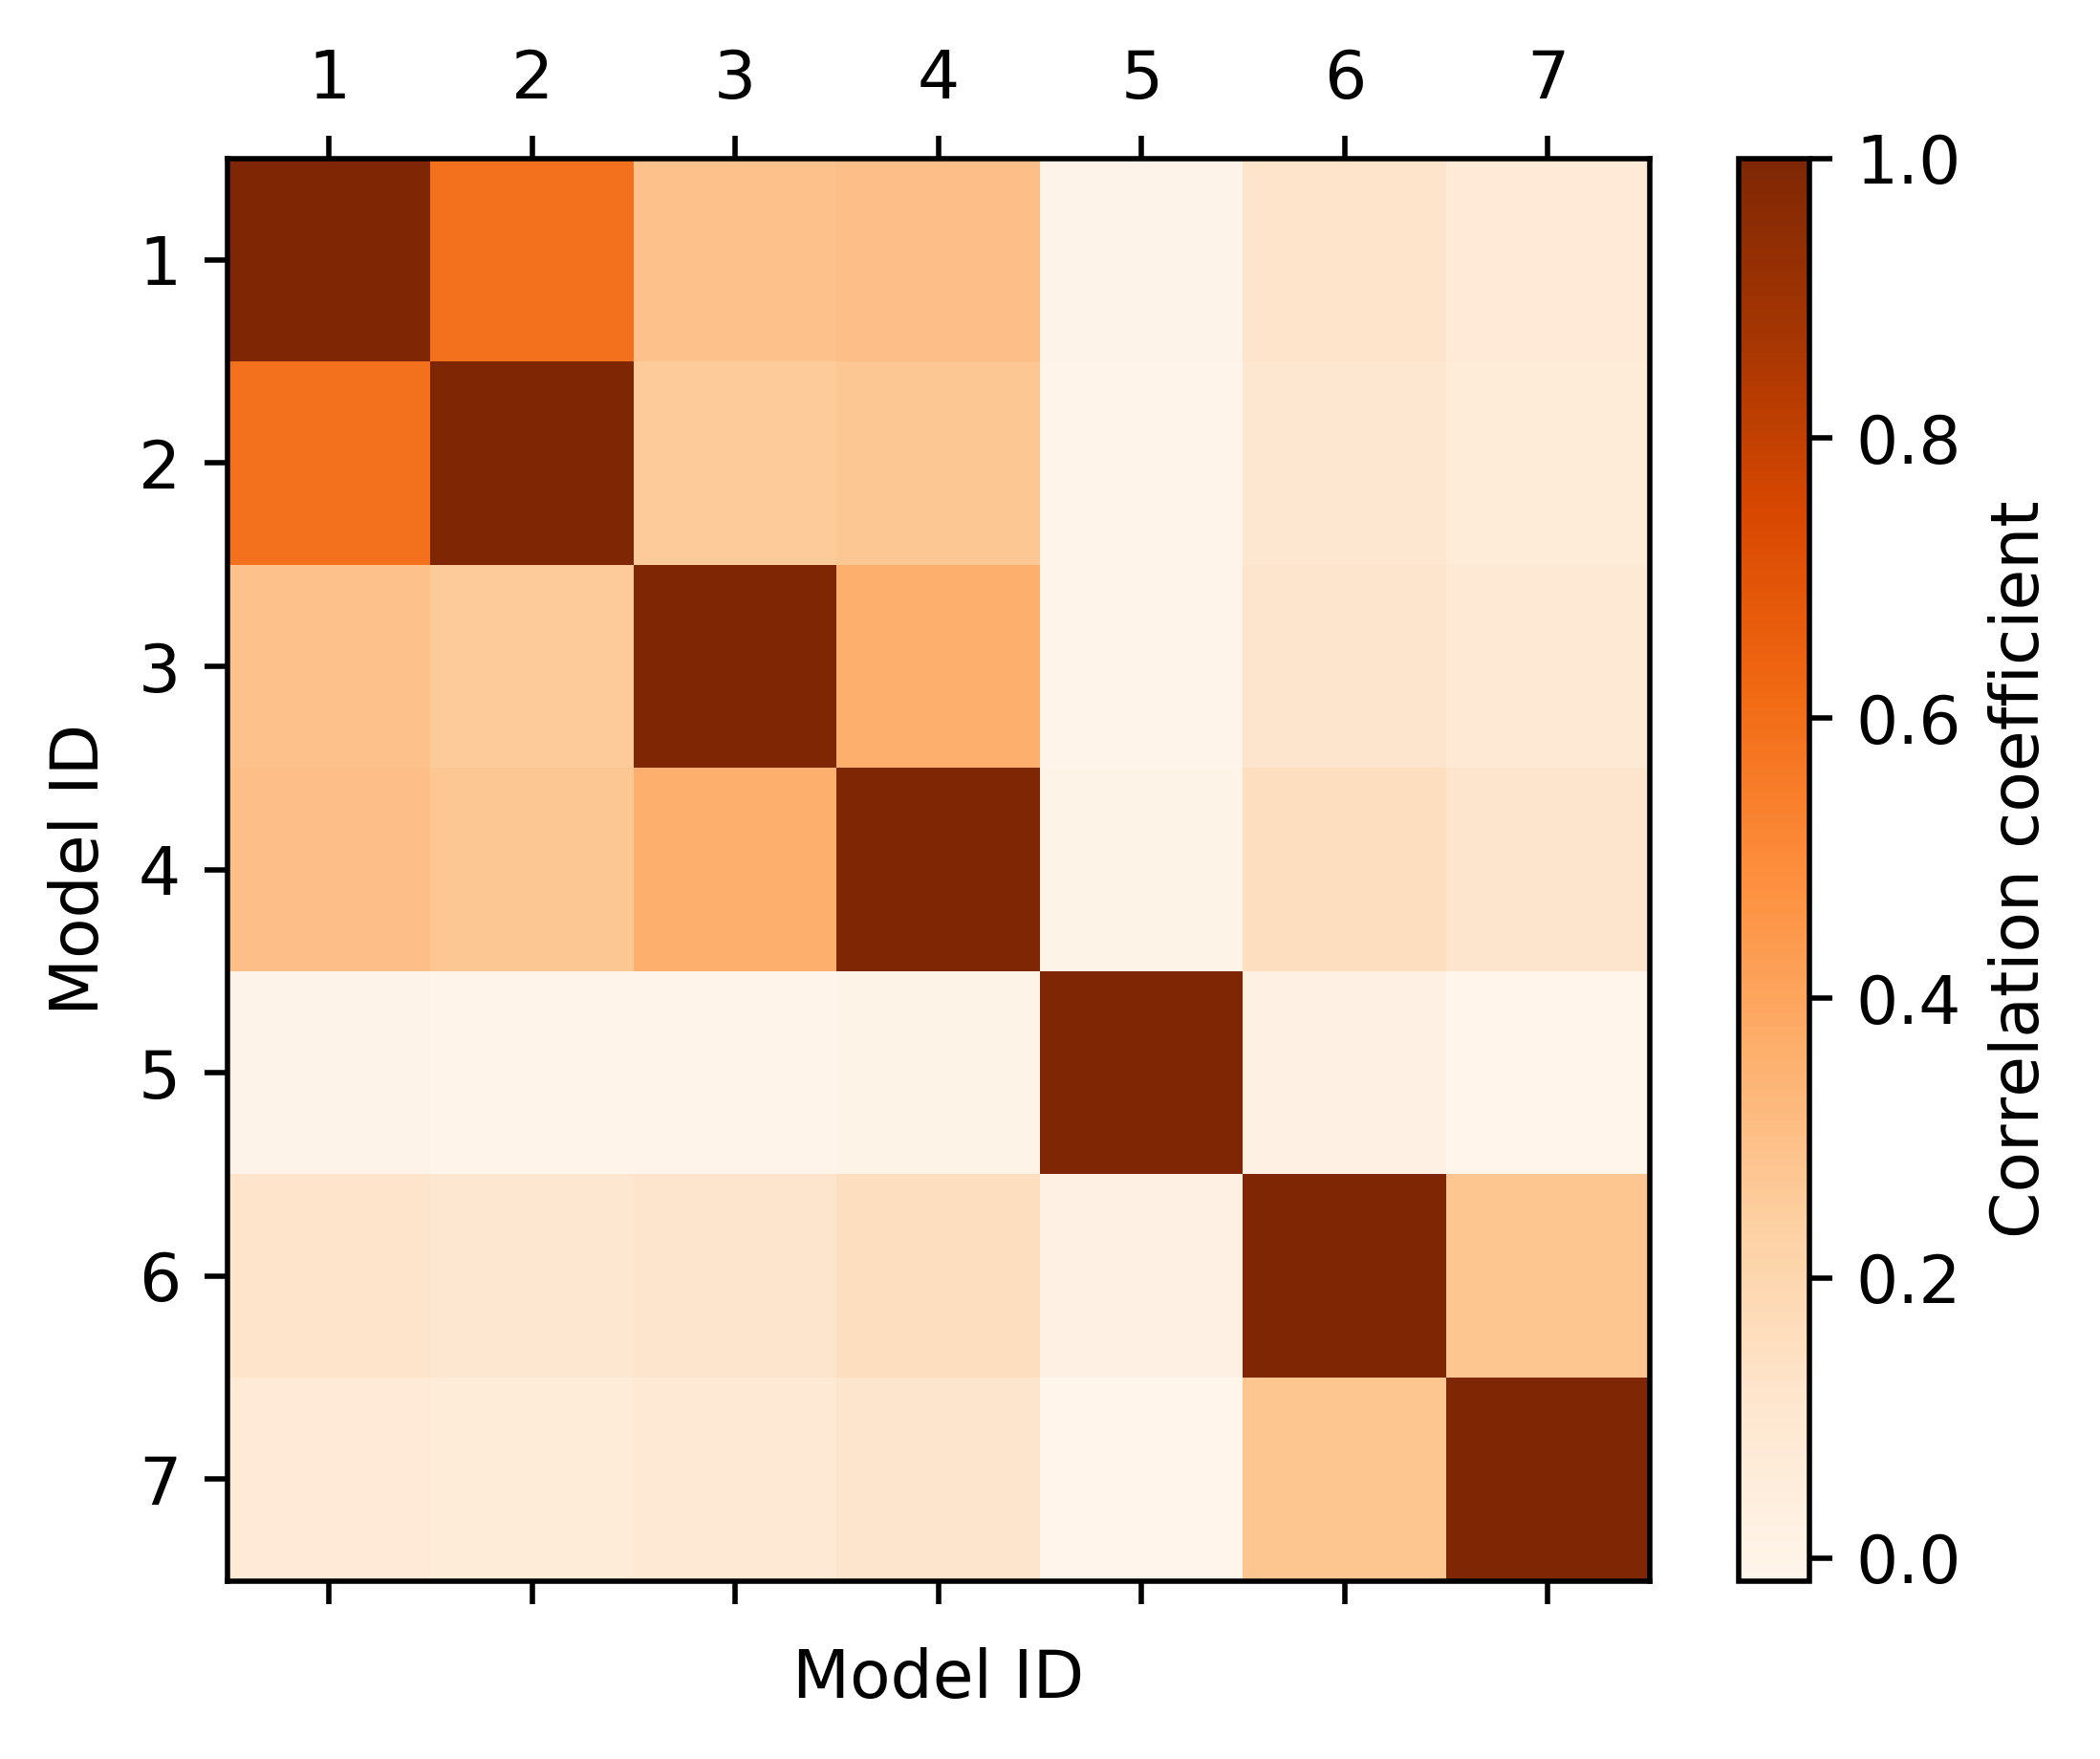
\includegraphics[width=0.35\textwidth]{fig/correlations.png}
	\caption{\textmd{Correlation matrix of the basic models, using the test data set.}}
	\label{fig:correlation_matrix}
\end{figure}